\documentclass[a4paper,ngerman,14pt]{scrartcl}
\usepackage[utf8]{inputenc}
\usepackage[ngerman]{babel}
\usepackage{graphicx}
\usepackage{setspace}
\usepackage{geometry}
\geometry{tmargin=2.7cm,bmargin=2cm,lmargin=2.3cm,rmargin=3cm}

\pagestyle{empty}

\renewcommand*{\familydefault}{\sfdefault}

\setlength{\unitlength}{1cm}

\begin{document}

\begin{picture}(0,0)
  \put(12.6,-0.1){%
    
\includegraphics[scale=0.15]{illustrationen/logo-uni}
  }
  \put(12,-18){%
    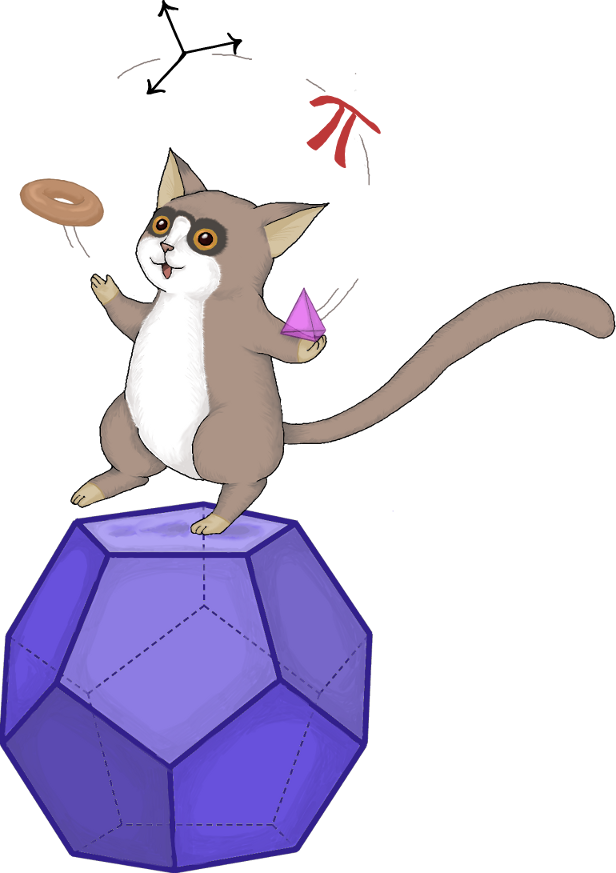
\includegraphics[scale=0.18]{illustrationen/cover}
  }
\end{picture}
\vspace{-3em}

\onehalfspacing

\begin{raggedright}
\Large\textbf{Matheschülerzirkel Augsburg}
\end{raggedright}
\vspace{0.2em}

\subsubsection*{Präsenzzirkel 5./6. Klasse}
\begin{tabbing}
  Mo \= 17:30–19:00, \= Raum 1007/L1: \= Alexander Engel \kill
  Mo \> 17:30–19:00, \> Raum 1007/L1: \> Alexander Engel \\
  Di \> 15:45–17:15, \> Raum 1008/L1: \> Stephanie Zapf \\
  Do \> 15:45–17:15, \> Raum 3008/L1: \> Carina Willbold
\end{tabbing}

\subsubsection*{Präsenzzirkel 7./8. Klasse}

\begin{tabbing}
  Mo \= 17:30–19:00, \= Raum 1007/L1: \= Alexander Engel \kill
  Mo \> 16:30–18:00, \> Raum 2006/L1: \> Simon Kapfer \\
  Mi \> 16:30–18:00, \> Raum 2006/L1: \> Kathrin Helmsauer \\
  Fr \> 16:30–18:00, \> Raum 1007/L1: \> Tim Baumann
\end{tabbing}

\subsubsection*{Präsenzzirkel 9./10. Klasse}

\begin{tabbing}
  Mo \= 17:30–19:00, \= Raum 1007/L1: \= Alexander Engel \kill
  Do \> 17:30–19:00, \> Raum 1009/L1: \> Sven Prüfer \\
  Di \> 14:15–16:15, \> Raum 2007/L1: \> Peter Uebele (Wettbewerbsvorbereitung)
\end{tabbing}

\subsubsection*{Präsenzzirkel 11./12. Klasse}

\begin{tabbing}
  Mo \= 17:30–19:00, \= Raum 1007/L1: \= Alexander Engel \kill
  Do \> 16:50–18:10, \> Raum 1005/L1: \> Philipp Düren \\
  Sa \> 14:30–16:00, \> Raum 2006/L1: \> Ingo Blechschmidt
\end{tabbing}

\subsubsection*{Korrespondenzzirkel}

\begin{tabbing}
  Wettbewerbsvorbereitung: \= \kill
  Klassenstufen 5 und 6: \> Johanna Fleckenstein \\
  Klassenstufen 7 und 8: \> Meru Alagalingam \\
  Klassenstufen 9 und 10: \> Christian Hübschmann \\
  Klassenstufen 11 und 12: \> Prof. Dr. Timo Schürg \\
  Wettbewerbsvorbereitung: \> Peter Uebele, Christopher Wulff \\
  \\
\small
Weitere Informationen: \textsl{http:/$\!$/www.math.uni-augsburg.de/schueler/mathezirkel/}
\end{tabbing}

\end{document}
